\documentclass[11pt,twoside,openright]{book}

% =======================================================================
% Preamble Konfigurasi Buku Dokumentasi LLM Bahasa Sangihe
% Disusun untuk Kompilasi menggunakan XeLaTeX
% =======================================================================

\usepackage{fontspec}
\usepackage{geometry}
\geometry{
    a4paper,
    total={160mm,245mm},
    left=28mm,
    right=22mm,
    top=28mm,
    bottom=25mm
}

% -----------------------------------------------------------------------
% Pengaturan Tipografi & Font Unicode Sangihe
% -----------------------------------------------------------------------
% Menggunakan Gentium Plus sebagai font utama (SIL International)
% Mendukung penuh seluruh karakter fonemis Sangihe:
% ạ, ẹ, ị, ọ, ụ, ě, ẹ̌, serta combining under-tilde U+1DCA pada l᷊
\setmainfont{Gentium Plus}

\setsansfont{Noto Sans}[
    Scale=0.92
]

\setmonofont{Noto Sans Mono}[
    Scale=0.88
]

% -----------------------------------------------------------------------
% Paket Pendukung Desain & Layout
% -----------------------------------------------------------------------
\usepackage{microtype}
\usepackage{amsmath,amssymb}
\usepackage{booktabs}
\usepackage{tabularx}
\usepackage{array}
\usepackage{graphicx}
\usepackage{xcolor}
\usepackage{fancyhdr}
\usepackage{titlesec}
\usepackage{enumitem}
\usepackage[most]{tcolorbox}
\usepackage{listings}
\usepackage{caption}
\usepackage{subcaption}
\usepackage{tikz}
\usepackage{pgfplots}
\pgfplotsset{compat=1.18}

% -----------------------------------------------------------------------
% Palet Warna Modern (Nord / Slate)
% -----------------------------------------------------------------------
\definecolor{primaryBlue}{HTML}{0284C7}
\definecolor{deepNavy}{HTML}{0F172A}
\definecolor{accentTeal}{HTML}{0D9488}
\definecolor{accentAmber}{HTML}{D97706}
\definecolor{accentRose}{HTML}{E11D48}
\definecolor{bgGray}{HTML}{F8FAFC}
\definecolor{borderGray}{HTML}{CBD5E1}
\definecolor{codeBg}{HTML}{F1F5F9}

% -----------------------------------------------------------------------
% Header & Footer
% -----------------------------------------------------------------------
\pagestyle{fancy}
\fancyhf{}
\fancyhead[LE,RO]{\thepage}
\fancyhead[LO]{\small\nouppercase{\rightmark}}
\fancyhead[RE]{\small\nouppercase{\leftmark}}
\renewcommand{\headrulewidth}{0.4pt}
\fancypagestyle{plain}{
    \fancyhf{}
    \fancyfoot[C]{\thepage}
    \renewcommand{\headrulewidth}{0pt}
}

% -----------------------------------------------------------------------
% Format Judul Bab & Seksi
% -----------------------------------------------------------------------
\titleformat{\chapter}[display]
  {\normalfont\sffamily\huge\bfseries\color{deepNavy}}
  {\filleft\Huge\sffamily\color{primaryBlue}\chaptertitlename\ \thechapter}
  {1ex}
  {\titlerule\vspace{1.5ex}\filright}
  [\vspace{1.5ex}\titlerule]

\titleformat{\section}
  {\normalfont\sffamily\Large\bfseries\color{deepNavy}}
  {\thesection}{1em}{}

\titleformat{\subsection}
  {\normalfont\sffamily\large\bfseries\color{primaryBlue}}
  {\thesubsection}{1em}{}

% -----------------------------------------------------------------------
% TColorBox untuk Kotak Informasi Teknis (Callouts)
% -----------------------------------------------------------------------
\newtcolorbox{infobox}[1][]{
    enhanced,
    colback=bgGray,
    colframe=primaryBlue,
    coltitle=white,
    fonttitle=\bfseries\sffamily,
    title={Catatan Arsitektur: #1},
    arc=3mm,
    boxrule=1pt,
    left=4mm, right=4mm, top=3mm, bottom=3mm,
    drop shadow=black!10!white
}

\newtcolorbox{linguisticbox}[1][]{
    enhanced,
    colback=bgGray,
    colframe=accentTeal,
    coltitle=white,
    fonttitle=\bfseries\sffamily,
    title={Kaidah Linguistik Sangihe: #1},
    arc=3mm,
    boxrule=1pt,
    left=4mm, right=4mm, top=3mm, bottom=3mm,
    drop shadow=black!10!white
}

\newtcolorbox{metricbox}[1][]{
    enhanced,
    colback=white,
    colframe=accentAmber,
    coltitle=white,
    fonttitle=\bfseries\sffamily,
    title={Metrik Evaluasi Empiris: #1},
    arc=3mm,
    boxrule=1pt,
    left=4mm, right=4mm, top=3mm, bottom=3mm,
    drop shadow=black!10!white
}

% -----------------------------------------------------------------------
% Konfigurasi Code Listings
% -----------------------------------------------------------------------
\lstset{
    backgroundcolor=\color{codeBg},
    basicstyle=\ttfamily\footnotesize,
    breaklines=true,
    breakatwhitespace=true,
    frame=single,
    rulecolor=\color{borderGray},
    numbers=left,
    numberstyle=\tiny\color{gray},
    keywordstyle=\color{primaryBlue}\bfseries,
    stringstyle=\color{accentTeal},
    commentstyle=\color{gray}\itshape,
    showstringspaces=false,
    tabsize=4,
    captionpos=b
}

% -----------------------------------------------------------------------
% Hyperref
% -----------------------------------------------------------------------
\usepackage[
    unicode=true,
    colorlinks=true,
    linkcolor=deepNavy,
    citecolor=primaryBlue,
    urlcolor=primaryBlue,
    bookmarksnumbered=true
]{hyperref}

% Auto-generated statistics from main translation engine project.
% Do NOT edit manually; updated via sync_project_status.py
\newcommand{\StatLastSyncDate}{03 November 2026}
\newcommand{\StatCorpusTotal}{30,296}
\newcommand{\StatCorpusBible}{29,671}
\newcommand{\StatCorpusDongeng}{28}
\newcommand{\StatCorpusHimbawo}{136}
\newcommand{\StatCorpusTigaKulano}{407}
\newcommand{\StatCorpusPercakapan}{54}
\newcommand{\StatLemmaTotal}{11,391}
\newcommand{\StatTrainPairs}{32,427}
\newcommand{\StatValPairs}{1,706}
\newcommand{\StatBenchmarkSamples}{150}
\newcommand{\StatBaseModel}{Qwen2.5-7B-Instruct}
\newcommand{\StatFinetunedModel}{sangiang:7b}
\newcommand{\StatModelCodename}{Sangiang}


\title{
    {\Huge\sffamily\bfseries Menghidupkan Bahasa di Era AI}\\[0.5em]
    {\Large\sffamily Kisah, Sains, dan Rekayasa di Balik Mesin Penerjemah Bahasa Sangihe}\\[1em]
    {\normalsize\itshape Membangun Jembatan Digital untuk Bahasa Daerah Nusantara}
}

\author{\textbf{Divisi DigiLab CMD}}
\date{\StatLastSyncDate}

\begin{document}

\frontmatter

% =======================================================================
% Halaman Depan (Title Page)
% =======================================================================
\begin{titlepage}
    \centering
    \vspace*{1.5cm}
    
    {\Huge\sffamily\bfseries\color{deepNavy} Menghidupkan Bahasa di Era AI}\\[0.6em]
    {\LARGE\sffamily\color{primaryBlue} Kisah, Sains, dan Rekayasa di Balik Mesin Penerjemah Sangiang}\\[1.5em]
    {\large\itshape Membangun Jembatan Digital untuk Bahasa Daerah Nusantara}
    
    \vspace{2.5cm}
    \begin{tcolorbox}[
        enhanced,
        colback=bgGray,
        colframe=primaryBlue,
        arc=2mm,
        width=0.85\textwidth,
        boxrule=0.8pt,
        halign=center
    ]
        {\small\sffamily\color{deepNavy}\textbf{Inisiator Proyek:}}\\[0.3em]
        {\Large\sffamily\bfseries\color{primaryBlue} Yayasan Cipta Mandala Dwipa}
    \end{tcolorbox}

    \vfill

    {\normalsize\sffamily Rekayasa Sistem AI dan Penerjemah:\\[0.4em] \textbf{\Large Divisi DigiLab CMD}}\\[1.5em]
    {\small\sffamily \StatLastSyncDate}
    \vspace*{1cm}
\end{titlepage}

% =======================================================================
% Halaman Copyright / Kolofon
% =======================================================================
\newpage
\thispagestyle{empty}
\vspace*{\fill}
\begin{flushleft}
    \small\sffamily
    \textbf{Menghidupkan Bahasa di Era AI:}\\
    \textit{Kisah, Sains, dan Rekayasa di Balik Mesin Penerjemah Bahasa Sangihe (Sangiang)}\\[0.8em]
    \rule{\textwidth}{0.6pt}\\[0.8em]
    
    \textbf{Inisiator Proyek:}\\
    \textbf{Yayasan Cipta Mandala Dwipa}\\[0.8em]
    
    \textbf{Rekayasa Sistem AI dan Penerjemah:}\\
    \textbf{Divisi DigiLab CMD}\\[0.8em]
    
    \textbf{Pernyataan Kepemilikan Hak Cipta:}\\
    \begin{itemize}[leftmargin=1.2em, itemsep=0.35em]
        \item \textbf{Yayasan Cipta Mandala Dwipa:} Pemilik hak cipta korpus terjemahan \textit{Kamus Sangihe-Indonesia}. Hak Cipta \copyright\ 2026 dilindungi oleh undang-undang.
        \item \textbf{Divisi DigiLab CMD:} Tim rekayasa sistem kecerdasan buatan (AI) dan penerjemah korpus.
        \item \textbf{Brill / KITLV (Koninklijk Instituut voor Taal-, Land- en Volkenkunde):} Pemilik hak cipta buku-buku kamus terkait, khususnya karya leksikografi klasik \textit{Sangihe-Nederlandsch Woordenboek} (1959) oleh K.G.F. Steller \& W.E. Aebersold.
        \item \textbf{Lembaga Alkitab Indonesia (LAI):} Pemilik hak cipta buku-buku teks Kitab Suci terkait, mencakup Alkitab Terjemahan Bahasa Sangihe, Terjemahan Baru (TB), dan Alkitab Bahasa Indonesia Masa Kini (BIMK).
    \end{itemize}
    \vspace{0.6em}
    
    \textbf{Misi \& Dedikasi:}\\
    Buku dan sistem teknologi ini dipersembahkan untuk masyarakat penutur Bahasa Sangihe di Kepulauan Sangihe, Sulawesi Utara, perantauan Nusa Utara, serta seluruh pecinta kebudayaan dan bahasa daerah Nusantara.\\[0.8em]
    
    \textbf{Tipografi \& Kompilasi Teknis:}\\
    Buku ini disusun dalam format \LaTeX\ dan dikompilasi menggunakan mesin Xe\LaTeX.\\
    Menggunakan jenis huruf \textit{Gentium Plus} karya SIL International untuk memastikan seluruh glif fonemis dan tanda diakritik ortografi Bahasa Sangihe (\d{a}, \d{e}, \v{\d{e}}, \v{e}, \d{i}, \d{o}, \d{u}, serta \textit{l᷊}) tercetak dengan sempurna.\\[0.8em]
    
    \textbf{Cetakan Digital:} Edisi Pertama -- \StatLastSyncDate\\
\end{flushleft}
\clearpage

\chapter*{Pengantar untuk Pembaca}
Buku ini ditulis bukan hanya untuk para peneliti kecerdasan buatan, melainkan untuk siapa saja yang mencintai bahasa daerah, kebudayaan Nusantara, dan ingin memahami bagaimana teknologi modern seperti \textit{Large Language Model} (LLM) dapat digunakan untuk menyelamatkan dan melestarikan warisan leluhur kita.

Proyek ini terwujud berkat inisiasi dan visi mulia dari \textbf{Yayasan Cipta Mandala Dwipa} yang berkomitmen pada pelestarian kebudayaan serta kemajuan peradaban literasi digital bahasa daerah. Setiap konsep teknis yang tampak rumit---mulai dari kecerdasan buatan, basis data, hingga struktur morfologi kata---akan dijelaskan dengan bahasa yang lugas, analogi sehari-hari, dan ilustrasi yang mudah dibayangkan.

\tableofcontents

\mainmatter

\part{Mengenal Bahasa Sangihe dan Tantangan Digitalnya}
\chapter{Menghidupkan Kembali Warisan Bahasa di Era Digital}

\section{Bahasa Sangihe: Mutiara Kebudayaan di Tapal Batas Utara}
Di ujung utara kepulauan Nusantara, terbentang gugusan pulau yang indah di wilayah Nusa Utara (Kabupaten Kepulauan Sangihe, Sulawesi Utara). Di tanah berombak inilah Bahasa Sangihe (\textit{Bahasa Sangir}) lahir, tumbuh, dan dituturkan secara turun-temurun oleh para pelaut ulung, penutur sastra lisan, dan masyarakat adat. Bahasa ini sarat dengan kearifan lokal, filosofi kehidupan bahari, serta karya sastra bernilai tinggi seperti wiracarita \textit{Sasahara} dan puisi epik \textit{Biong i Himbawo}.

Namun, seiring derasnya arus modernisasi dan peralihan generasi penutur muda ke bahasa pergaulan umum (Melayu Manado dan Bahasa Indonesia gaul), keberadaan bahasa daerah ini menghadapi tantangan yang nyata. Jika tidak ada upaya serius untuk mendokumentasikannya ke dalam bentuk digital dan menghadirkannya di gawai modern, bahasa yang kaya ini berisiko perlahan-lahan memudar dari percakapan sehari-hari.

\section{Tantangan AI: Mengapa Bahasa Daerah Kerap Tertinggal?}
Dalam beberapa tahun terakhir, dunia menyaksikan lompatan raksasa dalam teknologi kecerdasan buatan (\textit{Artificial Intelligence} / AI). Model-model bahasa besar (\textit{Large Language Model} atau LLM) seperti ChatGPT atau Qwen mampu menjawab pertanyaan rumit, menulis esai, bahkan menerjemahkan berbagai bahasa dunia dengan fasih.

\begin{infobox}[Analogi Perpustakaan Raksasa Dunia]
Bayangkan sebuah model AI modern seperti seorang sarjana pintar yang telah membaca miliaran buku dari perpustakaan terbesar dunia. Masalahnya, 95\% buku di perpustakaan tersebut ditulis dalam Bahasa Inggris, Mandarin, Spanyol, atau Bahasa Indonesia baku. Bahasa-bahasa daerah seperti Bahasa Sangihe hampir tidak pernah ia temukan di rak perpustakaan itu. Akibatnya, saat kita mengajaknya berbicara dalam Bahasa Sangihe, sang sarjana akan bingung atau sekadar menebak-nebak kata.
\end{infobox}

Dalam bidang linguistik komputasi, bahasa seperti Sangihe dikategorikan sebagai \textit{low-resource language} (bahasa berlindung sumber daya komputasi minim). Tantangan utamanya meliputi:
\begin{enumerate}
    \item \textbf{Kelangkaan Data Digital:} Tidak banyak situs web atau artikel daring yang memuat teks bahasa Sangihe dalam jumlah besar.
    \item \textbf{Kerumitan Tanda Diakritik:} Huruf vokal dalam bahasa Sangihe memiliki penanda khusus yang menentukan arti, yang kerap hilang saat diketik di ponsel pintar.
    \item \textbf{Morfologi yang Kaya:} Satu kata dasar bisa berubah wujud menjadi puluhan bentuk baru melalui awalan, sisipan di tengah kata, dan akhiran.
\end{enumerate}

\section{Misi Proyek: Membangun Mesin Penerjemah Cerdas}
Proyek ini lahir dengan sebuah cita-cita mulia namun terukur: \textbf{Membangun mesin penerjemah dua arah antara Bahasa Sangihe dan Bahasa Indonesia yang akurat, menghormati kaidah bahasa formal, dan dapat dijalankan di komputer biasa secara luring (offline) tanpa bergantung pada peladen cloud berbayar.}

Untuk mewujudkannya, proyek ini memadukan dua pendekatan teknologi mutakhir:
\begin{itemize}
    \item \textbf{Teknologi Hybrid RAG (\textit{Retrieval-Augmented Generation}):} Membekali sang model AI dengan "buku pintar" berupa kamus digital leksikon klasik dan bank ingatan kalimat paralel yang dapat ia buka setiap kali diminta menerjemahkan.
    \item \textbf{Pelatihan Khusus (\textit{Fine-Tuning}):} Melatih kembali saraf pemikiran model fondasi \texttt{\StatBaseModel} dengan puluhan ribu contoh kalimat terjemahan nyata agar ia memahami gaya, tata krama, dan jiwa Bahasa Sangihe.
\end{itemize}

Buku ini akan mengajak Anda menyusuri perjalanan lengkap bagaimana teknologi ini dirancang dari nol, langkah demi langkah, dengan penjelasan yang bersahabat bagi siapa saja.

\chapter{Seni Bunyi dan Rahasia Tanda Diakritik Sangihe}

\section{Mengapa Tanda Kecil Membawa Arti Besar?}
Dalam Bahasa Indonesia, kata \textit{tahu} (mengerti) dan \textit{tahu} (makanan berbahan kedelai) ditulis persis sama tanpa tanda baca khusus. Kita hanya bisa membedakannya lewat konteks kalimat. Namun, dalam Bahasa Sangihe, perbedaan bunyi vokal memiliki pengaruh yang sangat mendalam dan mutlak dalam menentukan arti suatu kata.

Untuk mengabadikan perbedaan bunyi tersebut ke dalam tulisan, para linguis dan penerjemah klasik (termasuk Dr. N. Adriani, K.G.F. Steller, dan W.E. Aebersold) merumuskan sistem ejaan dengan **tanda diakritik** (\textit{penanda aksen di atas atau di bawah huruf}).

\begin{linguisticbox}[Daftar Bunyi Khusus Bahasa Sangihe]
Bahasa Sangihe mengenal bunyi-bunyi khas yang tidak dimiliki oleh Bahasa Indonesia standar:
\begin{itemize}
    \item \textbf{Vokal Bertitik Bawah (\d{a}, \d{e}, \d{i}, \d{o}, \d{u}):} Menandakan vokal tertutup atau vokal panjang yang diucapkan dengan bibir lebih terkatup atau posisi lidah yang lebih tinggi.
    \item \textbf{Pepet (\v{e}):} Huruf $e$ lemah seperti bunyi huruf $e$ pada kata Indonesia \textit{sedap} atau \textit{segar}.
    \item \textbf{Kombinasi Bertitik-Pepet (\v{\d{e}}):} Bunyi vokal yang menggabungkan artikulasi tertutup dan nada sentak.
    \item \textbf{Lateral Terpalatisasi ($l^\sim$ / \textit{l᷊}):} Ditulis dengan huruf $l$ yang diberi tanda gelombang kecil di bawahnya (Unicode \texttt{U+1DCA}). Diucapkan seperti huruf $l$ yang lidahnya melengkung lembut ke langit-langit mulut.
\end{itemize}
\end{linguisticbox}

\section{Dilema Papan Ketik Modern: Masalah Mengetik di Ponsel}
Di zaman modern saat ini, hampir semua orang berkomunikasi menggunakan papan ketik standar (QWERTY) di ponsel pintar atau laptop. Di papan ketik tersebut, tidak ada tombol untuk huruf \textbf{\d{a}}, \textbf{\v{e}}, atau \textbf{l᷊}.

\begin{infobox}[Analogi Nada Musik Lagu Daerah]
Bayangkan sebuah partitur lagu daerah yang indah. Nada aslinya memiliki tanda nada tinggi, nada rendah, dan tanda jeda istirahat. Namun, saat dinyanyikan di jalanan tanpa teks, orang-orang hanya mengingat lirik dasarnya saja tanpa tanda not balok. Tugas mesin penerjemah pintar kita adalah seperti seorang guru paduan suara yang andal: meskipun pendengar hanya bersenandung datar (mengetik tanpa diakritik), sang guru tetap tahu nada yang benar dan mampu menuliskan kembali not balok lengkap dengan tanda lagunya secara sempurna.
\end{infobox}

Oleh karena itu, salah satu aturan emas (*core requirement*) yang ditetapkan sejak awal pembuatan sistem ini adalah:
\begin{center}
\textbf{“Input tanpa tanda diakritik harus diterima dengan lapang dada, namun keluaran hasil terjemahan Bahasa Sangihe harus tetap mengembalikan tanda diakritik yang lengkap dan akurat.”}
\end{center}

\section{Strategi Dua Jalur: Penormalan dan Pemulihan Diakritik}
Bagaimana sistem komputer kita mengatasi dilema ini? Kami merancang teknik yang disebut **Normalisasi Fonemis Dwiarah**:

\begin{enumerate}
    \item \textbf{Jalur Masuk (Penormalan Kata):} Saat pengguna mengetik kata \texttt{mebaese su waesu} (tanpa tanda apa pun), modul \texttt{normalizer.py} akan membersihkan huruf-huruf tersebut menjadi bentuk dasar. Huruf bertitik dan bertanda disetarakan ke huruf alfabet biasa ($a, e, i, o, u$). Tujuannya agar mesin pencari kamus dapat mencocokkannya dengan cepat di database leksikon.
    \item \textbf{Jalur Keluar (Pemulihan Diakritik):} Setelah model AI menerjemahkan kalimat, modul cerdas \texttt{DiacriticRestorer} akan memeriksa glosarium terverifikasi dan teks rujukan paralel. Modul ini secara otomatis menyisipkan kembali tanda diakritik yang sah, sehingga kata berubah kembali menjadi ejaan formal: \textbf{\textit{měbaes\d{e}\v{} su waes-u}}.
\end{enumerate}

Dengan rancangan ini, pengguna yang awam tidak perlu repot mencari simbol tersembunyi di papan ketik saat mengetik kalimat, namun hasil terjemahan yang dihasilkan tetap menjunjung tinggi kehormatan ortografi asli Bahasa Sangihe.

\chapter{Morfologi Sangihe: Seni Membongkar dan Menyusun Kata}

\section{Morfologi: Mengapa Kata Dasar Bisa Berubah Wujud?}
Dalam ilmu bahasa, **morfologi** adalah studi tentang bagaimana kata dibentuk dari potongan-potongan makna terkecil. Jika dalam Bahasa Indonesia kita mengenal kata dasar \textit{ajar} yang bisa menjadi \textit{belajar, mengajar, terpelajar}, maka dalam Bahasa Sangihe variasinya jauh lebih kaya dan dinamis.

\begin{infobox}[Analogi Bongkar Pasang Pakaian]
Bayangkan sebuah kata dasar seperti sesosok tubuh manusia. Morfologi adalah seni memakaikan pakaian pada tubuh tersebut:
\begin{itemize}
    \item Memakaikan topi di kepala disebut \textbf{Awalan (Prefiks)}, seperti \textit{mě-}, \textit{ma-}, atau \textit{ipang-}.
    \item Memakaikan sabuk di tengah pinggang disebut \textbf{Sisipan (Infiks)}, seperti menyisipkan suku kata \textit{-um-} atau \textit{-in-} tepat di tengah perut kata!
    \item Memakaikan sepatu di kaki disebut \textbf{Akhiran (Sufiks)}, seperti \textit{-ang}, \textit{-eng}, atau \textit{-e}.
    \item Mengajak bayangannya ikut berjalan bersama disebut \textbf{Pengulangan (Reduplikasi)}.
\end{itemize}
Tugas modul komputer kita (\texttt{stemmer.py}) adalah seperti seorang detektif yang melihat seseorang berpakaian lengkap, lalu menanggalkan topinya, melepas sabuknya, dan mencopot sepatunya agar dapat mengenali siapa sosok orang (kata dasar) yang sebenarnya!
\end{infobox}

\section{Keunikan Sisipan di Dalam Perut Kata}
Salah satu ciri khas rumpun bahasa Filipina dan Austronesia utara yang diwarisi oleh Bahasa Sangihe adalah keberadaan **infiks** (sisipan). Di sebagian besar bahasa dunia, imbuhan hanya dipasang di depan atau di belakang kata. Namun di Bahasa Sangihe, imbuhan diselipkan ke sela-sela huruf pertama dan kedua kata dasar:

\begin{linguisticbox}[Contoh Sisipan -um- dan -in-]
Perhatikan bagaimana kata dasar bertransformasi saat disisipi makna tindakan atau kala lampau:
\begin{itemize}
    \item Kata dasar: \textbf{tampa} (\textit{tempat / tiba}) $\rightarrow$ Disisipi \textit{-um-} di antara $t$ dan $a$ $\rightarrow$ \textbf{t-um-ampa} (\textit{sedang tiba / datang melangkah}).
    \item Kata dasar: \textbf{koro} (\textit{bakar}) $\rightarrow$ Disisipi \textit{-in-} $\rightarrow$ \textbf{k-in-oro} (\textit{telah dibakar}).
\end{itemize}
Jika modul pencari di komputer tidak memahami aturan sisipan ini, komputer akan mencari kata \textit{tumampa} di kamus dan tidak akan pernah menemukannya, karena kata tersebut terdaftar di bawah huruf T (\textit{tampa}), bukan huruf T-U!
\end{linguisticbox}

\section{Hukum Alih Bunyi: Studi Kasus Nyata Kata \textit{Waes}}
Dalam perjalanan pengembangan translation engine ini, kami menemukan sebuah kasus menarik yang membuktikan betapa pentingnya pemahaman morfologi yang mendalam.

Dalam dongeng klasik Sangihe, terdapat sebuah kalimat terkenal:
\begin{center}
\textit{“Mahi i\d{a}ko m\v{e}baes\v{\d{e}} su \textbf{waes-u}.”}
\end{center}
Awalnya, sistem penerjemah menerjemahkan kata \textbf{waes-u} dengan arti "kemarau-mu", padahal arti yang tepat dalam konteks cerita binatang tersebut adalah **"sarang-mu"**! Mengapa kebingungan ini bisa terjadi?

\begin{enumerate}
    \item Kata aslinya berbunyi \textbf{baes\v{\d{e}}} (lema nomor 331 di kamus Steller-Aebersold).
    \item Saat kata benda ini diberi kata ganti milik \textit{-u} ("milikmu"), bahasa Sangihe memberlakukan hukum fonemis:
    \begin{itemize}
        \item Konsonan bibir $b$ bermutasi melunak menjadi $w$ ($b \leftrightarrow w$).
        \item Huruf vokal gema (\textit{echo vowel}) di ujung kata luruh, menyisakan akar \textit{waes}.
        \item Ditambahkan akhiran \textit{-u}, menjadi \textbf{waes-u}.
    \end{itemize}
\end{enumerate}

Dengan menanamkan aturan alih bunyi ini ke dalam berkas \texttt{morphology/stemmer.py}, komputer kini secara otomatis tahu bahwa kata \textit{waes} berasal dari lema asli \textbf{\textit{baes\v{\d{e}}}}. Mesin pencari kamus pun berhasil menemukan arti lema yang sebenarnya di dalam database hanya dalam waktu kurang dari 2 milidetik!


\part{Mengumpulkan Harta Karun Kata: Korpus \& Kamus}
\chapter{Mengumpulkan Harta Karun Kata: Korpus \& Kamus Klasik}

\section{Bahan Bakar Utama Kecerdasan Buatan: Data Paralel}
Sebuah mobil secanggih apa pun tidak akan dapat melaju tanpa bahan bakar. Demikian pula dengan kecerdasan buatan: model AI secanggih apa pun tidak akan bisa menerjemahkan bahasa tanpa adanya data contoh kalimat yang benar.

Dalam dunia penerjemahan mesin, data paling berharga disebut **Korpus Paralel** (\textit{Parallel Corpus}).

\begin{infobox}[Analogi Buku Dua Bahasa dan Teks Film]
Bayangkan sebuah buku cerita yang di halaman kirinya dicetak dalam Bahasa Sangihe, dan tepat di halaman kanannya dicetak terjemahan resminya dalam Bahasa Indonesia kalimat demi kalimat. Atau bayangkan sebuah film yang menampilkan dua baris terjemahan teks (subtitle) sekaligus di layar. Dengan membandingkan ribuan pasangan kalimat tersebut, kecerdasan buatan dapat mempelajari bagaimana frasa tertentu dialihbahasakan secara alami.
\end{infobox}

\section{Lima Sumber Daya Utama Proyek Ini}
Proyek ini mengintegrasikan lima warisan dokumen besar yang telah didigitisasi:

\subsection{1. Kamus Klasik Steller-Aebersold (\StatLemmaTotal{} Lema)}
Kamus monumental \textit{Sangihe-Nederlandsch Woordenboek} karya K.G.F. Steller dan W.E. Aebersold (1959) diterbitkan di bawah naungan Koninklijk Instituut voor Taal-, Land- en Volkenkunde (KITLV), dengan hak cipta buku dipegang oleh \textbf{Brill / KITLV}. 

Adapun korpus terjemahan kamus tersebut ke dalam Bahasa Indonesia---yang dikerjakan secara cermat dan komprehensif oleh tim penerjemah \textbf{Divisi DigiLab CMD} dan menjadi basis leksikal komputasi dalam proyek ini---merupakan hak cipta milik \textbf{Yayasan Cipta Mandala Dwipa}. Di dalam sistem, data ini dimuat dari basis data SQLite \texttt{sarindi.sqlite} yang mencakup:
\begin{itemize}
    \item \textbf{\StatLemmaTotal{} lema utama} lengkap dengan tanda diakritik fonemis dan penjelasan arti rinci.
    \item \textbf{Indeks Balik Bahasa Indonesia (\textit{id\_index}):} Memungkinkan kita mencari padanan kata Sangihe dari sudut pandang kosakata Bahasa Indonesia.
    \item \textbf{Pencarian Teks Cepat (SQLite FTS5):} Memungkinkan komputer menemukan lema yang cocok dalam hitungan sepersekian milidetik.
\end{itemize}

\subsection{2. Teks Paralel Kitab Suci Sangihe (\StatCorpusBible{} Ayat)}
Naskah terjemahan Alkitab Bahasa Sangihe yang disandingkan berdampingan dengan Alkitab Terjemahan Baru (TB) dan Bahasa Indonesia Masa Kini (BIMK). Hak cipta dari seluruh naskah dan buku teks Kitab Suci ini dipegang oleh \textbf{Lembaga Alkitab Indonesia (LAI)}. Sumber ini menyumbang lebih dari 29 ribu pasangan ayat dengan register bahasa formal, tata kalimat yang tertib, dan diakritik yang terjaga rapi.

\subsection{3. Sastra Klasik: Dongeng Sasahara \& Wiracarita Himbawo}
Untuk melengkapi ragam bahasa percakapan, metafora bahari, dan folklor tradisional, proyek ini memasukkan:
\begin{itemize}
    \item \textbf{27 Bab Dongeng Klasik Sangihe (\StatCorpusDongeng{} Kalimat):} Kisah binatang, fabel moral, dan legenda rakyat (seperti kisah Gurita dan Ular Laut).
    \item \textbf{Puisi Epik \textit{Biong i Himbawo} (\StatCorpusHimbawo{} Larik):} Nyanyian kepahlawanan dengan struktur persajakan puitis tingkat tinggi.
\end{itemize}

\subsection{4. Sastra Folklor Daerah: \textit{Tiga Kulano dari Dagho} (\StatCorpusTigaKulano{} Pasangan Kalimat)}
Sebagai terobosan mutakhir untuk memutus ketergantungan model terhadap domain religius (bias 99\% teks Alkitab), proyek ini mengintegrasikan buku kumpulan cerita rakyat dwibahasa \textit{Tiga Kulano dari Dagho} (Paul Nebath dkk., Departemen Pendidikan dan Kebudayaan, 1983). Korpus ini mencakup 14 bab kisah kepahlawanan, fabel satwa, mitologi laut, dan asal-usul tanjung yang tersebar di wilayah kepulauan:
\begin{itemize}
    \item \textbf{10 Cerita Sangihe Besar (286 Pasangan):} Termasuk wiracarita \textit{Gumansalangi}, putri legendaris \textit{Tomatiti}, pahlawan bahari \textit{Tiga Orang Pemberani dari Dagho}, \textit{Ompung} (dewa lautan), serta fabel satwa jenaka \textit{Kera dan Bangau}.
    \item \textbf{2 Cerita Bahasa Talaud (70 Pasangan):} Kisah manusia pertama di Pulau Karakelang (\textit{Alamona Ntaumata Ntaloda}) dan hikmah anak yang durhaka (\textit{Battiu Anao}).
    \item \textbf{1 Cerita Dialek Tagulandang (32 Pasangan):} Legenda terbentuknya tanjung terputus (\textit{Tonggeng Napoto}).
    \item \textbf{1 Cerita Dialek Siau (19 Pasangan):} Fabel musyawarah satwa \textit{Kina Hetung dingangu Manu Banggiung}.
\end{itemize}

\begin{infobox}[Pemulihan Filologis \& Rekonstruksi Halaman Tertukar]
Pada buku cetakan fisik tahun 1983, keterbatasan teknologi cetak saat itu memaksa penyunting menambahkan tanda-tanda diakritik menggunakan coretan pena manual di atas ketikan mesin tik, yang saat dipindai melalui OCR menghasilkan ribuan derau karakter. Selain itu, ditemukan anomali perwajahan kritis di mana potongan naskah Bahasa Sangihe antara Cerita 7 (\textit{Walawo, Urang, Lipang...}) dan Cerita 12 (\textit{Datu I Ralero}) tertukar halamannya pada lembaran cetak. 

Melalui pipeline restorasi berbasis leksikon Steller-Aebersold (\texttt{scripts/process\_tiga\_kulano.py}) dan algoritma \textit{Dynamic Programming Sentence Alignment}, kedua naskah berhasil disambung kembali sesuai koherensi plot aslinya, serta dibersihkan ke dalam ortografi fonemis baku lengkap dengan konsonan kepak retrofleks (\textit{l᷊}) dan vokal pepet (\textit{ě, ẹ̌}).
\end{infobox}

\subsection{5. Korpus Percakapan Sehari-Hari (\StatCorpusPercakapan{} Pasangan Kalimat)}
Untuk menjembatani model dengan situasi percakapan nyata di dunia modern, proyek ini menyaring dan menyelaraskan data kosakata percakapan dari sumber-sumber web terbuka (\texttt{data/web/}) serta ungkapan pragmatis kesantunan masyarakat kontemporer. Korpus ini dikurasi secara cermat melalui skrip \texttt{scripts/process\_web\_conversations.py}:
\begin{itemize}
    \item \textbf{Salam Waktu \& Sapaan:} Ungkapan salam formal dan santai seperti \textit{Salamate měhěbị} (selamat pagi), \textit{Salamate ěllong darua} (selamat siang), \textit{Salamate sělẹ̌} (selamat sore), dan \textit{Salamate hěbi} (selamat malam).
    \item \textbf{Pragmatik Kesantunan:} Frasa penting dalam interaksi sosial seperti \textit{Tarima kasehẹ̌} (terima kasih), \textit{Makiangsingkatẹ̌} (terima kasih banyak), \textit{Kapurane iạ} (maafkan saya), \textit{Tabea} (permisi), dan \textit{Pariurung} (silakan).
    \item \textbf{Tanya Jawab Percakapan:} Pola tanya jawab lazim seperti kabar (\textit{Kere habarẹ̌?}), asal (\textit{Bọu apa i kau?}), tujuan (\textit{Sarang apa i kau?}), nama (\textit{Isai arengu?}), serta jamuan makan (\textit{Ndaị e kumâng!}).
    \item \textbf{Panggilan Budaya:} Panggilan kehormatan dan kasih sayang khas suku Sangihe seperti \textit{Ungke / Opo} (pemuda) dan \textit{Wawu} (pemudi).
\end{itemize}
Kehadiran korpus percakapan ini memberikan penahan (*pragmatic anchor*) yang esensial agar bot percakapan Sangiang (Port 2026) dapat merespons tegur sapa warga dengan luwes, santun, dan alami tanpa mengeluarkan respons yang melantur.

\section{Totalitas Bank Memori Paralel}
Melalui modul pengindeks cerdas (\texttt{retrieval/indexer.py}), seluruh data ini dilebur dan disimpan dalam satu basis data terpadu \texttt{parallel\_corpus.sqlite}. Kini sistem memiliki total \textbf{\StatCorpusTotal{} pasangan kalimat rujukan} yang siap dipanggil kapan saja oleh mesin penerjemah.

\chapter{Membersihkan Butiran Emas: Normalisasi dan Pre-processing}

\section{Mengapa Teks Mentah Tidak Boleh Langsung Diproses?}
Dalam pepatah ilmu data, dikenal prinsip terkenal: \textit{“Garbage In, Garbage Out”} (jika data yang dimasukkan berantakan, maka hasil yang dikeluarkan komputer juga akan kacau). Sebelum sebuah kamus atau teks kalimat dapat dipakai oleh kecerdasan buatan, teks tersebut harus melalui proses pembersihan dan perapian (*pre-processing*).

\begin{infobox}[Analogi Menyaring Pasir Emas]
Menambang data dari buku-buku tua mirip dengan mendulang pasir emas di sungai. Di dalam pasir tersebut, terdapat butiran emas berharga (kata-kata bermakna), tetapi juga terdapat kerikil, lumpur, dan dedaunan (tanda kutip ganda yang miring, spasi berlebih, huruf besar-kecil yang tidak konsisten). Modul pre-processing kita bertindak sebagai ayakan halus yang mencuci bersih data mentah sehingga yang tersisa hanyalah kosakata murni yang siap diolah.
\end{infobox}

\section{Langkah-Langkah Pembersihan Teks}
Modul \texttt{morphology/normalizer.py} menjalankan beberapa tugas penting:

\begin{enumerate}
    \item \textbf{Penyatuan Tanda Petik dan Glotal (\textit{Apostrophe Standardization}):} Dalam naskah ketikan, tanda petik sering bervariasi antara tanda petik tegak (\texttt{'}), petik miring (\texttt{’}), atau aksen (\texttt{`}). Modul kami menyatukan semuanya ke satu standar agar pencarian tidak meleset.
    \item \textbf{Penormalan Spasi \& Tanda Baca:} Menghilangkan spasi ganda, merapikan tanda titik-koma, serta memisahkan tanda baca yang menempel pada kata tanpa merusak arti.
    \item \textbf{Penyaringan Kata Tugas (\textit{Stopwords Filtering}):} Dalam percakapan, kata-kata sambung pendek seperti \textit{su} (di/pada), \textit{u} (dari/milik), \textit{i} (si/penanda nama orang), dan \textit{k\d{u}} (dan/lalu) muncul ribuan kali. Jika komputer mencari arti kata \textit{su} di kamus setiap kali menerjemahkan, proses akan menjadi sangat lambat tanpa memberikan nilai tambah. Sistem kami secara cerdas memfilter kata-kata tugas umum ini saat mencari leksikon utama.
\end{enumerate}

Dengan langkah-langkah di atas, mesin penerjemah dapat berkonsentrasi penuh pada kata-kata kunci pembawa pesan utama dalam kalimat.

\chapter{Ujian yang Jujur: Tolok Ukur Benchmark \& Anti-Kebocoran Data}

\section{Mengapa Kita Butuh Ujian yang Independen?}
Bagaimana kita tahu bahwa sistem penerjemah AI kita benar-benar pandai menerjemahkan, dan bukan sekadar "menghafal mati" kalimat-kalimat yang pernah ia lihat?

\begin{infobox}[Analogi Soal Ujian Akhir Sekolah]
Bayangkan seorang guru yang sedang mendidik muridnya menjelang ujian nasional. Selama berbulan-bulan di kelas, sang guru memberikan ratusan latihan soal (ini adalah \textbf{Data Latih / Training Set}). Namun, saat hari ujian tiba, sang guru harus mengunci lembar soal ujian akhir di laci tertutup dan tidak boleh membocorkannya kepada murid (ini adalah \textbf{Data Uji / Test Benchmark}). 

Jika seorang murid mendapatkan nilai 100 karena sebelumnya sudah melihat kunci jawaban soal ujian, nilai tersebut adalah nilai palsu (\textit{data leakage}). Tetapi jika murid tersebut mampu menjawab soal-soal baru yang belum pernah ia lihat sama sekali, barulah kita yakin bahwa ia benar-benar cerdas!
\end{infobox}

\section{Menyusun 150 Kalimat Uji Acuan}
Untuk menguji kemampuan sistem secara objektif, modul \texttt{benchmark/generate\_testset.py} menyaring **\StatBenchmarkSamples{} kalimat acuan** pilihan dari seluruh korpus data kita. Kalimat-kalimat ini dipilih dengan metode cuplikan berlapis (*stratified sampling*) yang mencakup:
\begin{itemize}
    \item Kalimat pendek (sapaan dan ujaran ringkas).
    \item Kalimat panjang dengan anak kalimat majemuk.
    \item Kalimat dengan kepadatan tanda diakritik tinggi (\d{a}, \d{e}, \v{e}, l᷊).
    \item Representasi berimbang dari ketiga domain (teks Alkitab, fabel dongeng rakyat, dan puitika Himbawo).
\end{itemize}

Seluruh 150 kalimat ini disimpan secara terisolasi di dalam berkas \texttt{benchmark/testset.json}.

\section{Prinsip Ketat Anti-Kebocoran Data (\textit{Anti-Leakage})}
Saat modul \texttt{training/prepare\_dataset.py} mengekstrak data untuk melatih model bahasa, sistem secara otomatis membaca seluruh identitas unik (ID) dari ke-150 kalimat uji tersebut dan **mengecualikannya secara mutlak** dari kumpulan data latih.

Dengan demikian, ketika model AI diuji di akhir nanti, model tersebut benar-benar diuji dengan kalimat-kalimat yang belum pernah ia temui selama sesi latihannya di komputer.

\section{Tiga Rapor Penilaian Kualitas}
Untuk mengukur seberapa bagus terjemahan yang dihasilkan, kami menggunakan tiga metrik internasional yang dihitung secara matematis oleh modul \texttt{benchmark/evaluate.py}:
\begin{enumerate}
    \item \textbf{Skor BLEU (\textit{Bilingual Evaluation Understudy}):} Mengukur seberapa banyak kecocokan urutan kata (1 kata, 2 kata, hingga 4 kata berturut-turut) antara hasil terjemahan AI dengan terjemahan resmi pakar manusia. Semakin tinggi skornya (skala 0--100), semakin mirip hasil terjemahannya dengan bahasa manusia.
    \item \textbf{Skor chrF++ (\textit{Character n-gram F-score}):} Berbeda dengan BLEU yang mencocokkan kata per kata, chrF++ mencocokkan susunan huruf demi huruf. Metrik ini sangat adil untuk bahasa daerah yang memiliki banyak imbuhan dan tanda diakritik.
    \item \textbf{Rasio Kepadatan Diakritik (\textit{Diacritic Density Ratio}):} Menghitung apakah jumlah tanda diakritik pada terjemahan Sangihe sesuai dengan standar ortografi resmi ataukah huruf-hurufnya gundul tanpa aksen.
\end{enumerate}


\part{Arsitektur Cerdas: Teknologi Hybrid RAG}
\chapter{Arsitektur Cerdas: Mengapa Memilih Teknologi Hybrid RAG?}

\section{Dua Cara Belajar: Menghafal Mati vs Ujian Buka Buku}
Ketika manusia belajar bahasa asing, ada dua cara yang bisa ditempuh:
\begin{enumerate}
    \item \textbf{Menghafal Seluruh Kamus di Luar Kepala:} Menghafal ribuan kata dan jutaan kalimat sampai kepala pusing. Masalahnya, ingatan manusia (dan memori parameter AI) bisa salah ingat, mencampuradukkan kata, atau mengarang fakta yang tidak ada (dalam istilah AI disebut \textit{halusinasi}).
    \item \textbf{Ujian Sistem Buka Buku (\textit{Open-Book Examination}):} Belajar memahami tata bahasa dan pola kalimat, lalu saat bertugas menerjemahkan dokumen, kita meletakkan sebuah kamus besar dan catatan arsip terjemahan terdahulu di atas meja kerja kita.
\end{enumerate}

\begin{infobox}[Prinsip RAG: Retrieval-Augmented Generation]
Teknologi **RAG** (\textit{Pengambilan Informasi yang Memperkaya Generasi Teks}) adalah perwujudan digital dari konsep ujian buka buku. Setiap kali ada pengguna yang mengetik kalimat untuk diterjemahkan, sistem komputer tidak langsung menyuruh model AI mengarang jawaban. Sistem akan terlebih dahulu menjadi "asisten perpustakaan" yang gesit: membuka arsip kamus, mengambil halaman rujukan yang cocok, lalu menyerahkan kutipan rujukan tersebut ke hadapan model AI seraya berkata: \textit{“Ini kalimat yang diminta, dan ini arti kata-kata resminya dari kamus. Terjemahkanlah sekarang berdasarkan rujukan ini!”}
\end{infobox}

\section{Mengapa Harus \textit{Hybrid} (Campuran Dua Tingkat)?}
Dalam penerjemahan bahasa daerah, mencari rujukan hanya dari satu sumber sering kali tidak cukup. Oleh karena itu, arsitektur kami dinamakan **Hybrid RAG** karena menggabungkan dua tingkat rujukan sekaligus:

\begin{enumerate}
    \item \textbf{Tingkat 1: Rujukan Kata Dasar (Leksikon Steller-Aebersold)} \\
    Sistem mencari arti setiap kata penting yang ada dalam kalimat. Jika ada kata \textit{bal\d{o}to}, kamus akan membisikkan bahwa artinya adalah \textit{ular laut}; jika ada kata \textit{kuhita}, artinya adalah \textit{gurita}. Ini memastikan model AI tidak salah mengartikan kosakata langka.
    \item \textbf{Tingkat 2: Rujukan Kalimat Utuh (\textit{Translation Memory})} \\
    Sistem mencari kalimat dalam basis data 29 ribu ayat yang memiliki susunan kata paling mirip dengan kalimat input. Ini memberikan contoh nyata bagaimana menyusun tata krama, intonasi, dan struktur frasa yang sopan.
\end{enumerate}

Dengan menyatukan kedua rujukan ini ke dalam satu lembar panduan singkat, model AI \texttt{\StatBaseModel} dapat menghasilkan terjemahan yang tepat sasaran, fasih, dan memiliki dasar filologis yang dapat dipertanggungjawabkan.

\chapter{Mesin Pencari Secepat Kilat: Menyelamatkan Komputer dari Kemacetan Memori}

\section{Tantangan Nyata di Komputer Pribadi}
Banyak penelitian kecerdasan buatan berasumsi bahwa sistem akan dijalankan di pusat data raksasa milik korporasi teknologi dengan lusinan kartu grafis (GPU) seharga ratusan juta rupiah. Namun, proyek ini dirancang dengan prinsip kemandirian: **harus bisa berjalan di komputer kerja biasa (komputer meja atau laptop dengan prosesor Intel dan memori RAM 32 GB) tanpa kartu grafis khusus.**

Menjalankan model kecerdasan buatan berukuran 7 miliar parameter (\texttt{Qwen2.5:7b}) di atas prosesor biasa (CPU) memiliki tantangan tersendiri: setiap detiknya sangat berharga.

\section{Kisah Kemacetan Memori: Tragedi Model yang Terus Tergusur}
Di tahap awal eksperimen, kami mencoba menggunakan metode pencarian vektor modern bernama \textit{Dense Embedding} (menggunakan model khusus bernama \texttt{bge-m3}). Namun, sebuah fenomena mengejutkan terjadi: setiap kali pengguna mengirimkan satu kalimat panjang, sistem tiba-tiba membeku selama dua menit lebih lalu menampilkan pesan galat: \textit{“Ollama Timeout”}!

Apa yang sebenarnya terjadi di dalam "otak" komputer?

\begin{infobox}[Analogi Meja Kerja yang Sempit]
Bayangkan Anda memiliki meja belajar kecil yang hanya muat satu buku ensiklopedia raksasa setebal 5.000 halaman (\textbf{Model Bahasa Qwen}). 
Tiba-tiba, seorang asisten datang dan meminta Anda membuka buku kamus saku kecil (\textbf{Model Pencari Vektor BGE-M3}). Karena meja Anda tidak muat dua buku sekaligus, Anda terpaksa:
\begin{enumerate}
    \item Mengangkat buku raksasa 5.000 halaman itu ke lemari gudang (butuh waktu 15 detik).
    \item Meletakkan buku kamus saku di atas meja untuk mencari satu kata (butuh waktu 1 detik).
    \item Mengangkat kembali buku kamus saku ke lemari, lalu berjalan ke gudang memikul kembali buku raksasa 5.000 halaman itu ke atas meja (butuh waktu 45 detik!).
\end{enumerate}
Hanya untuk mencari satu kata, Anda menghabiskan waktu semenit lebih hanya untuk bolak-balik mengangkat buku! Dalam ilmu komputer, fenomena ini dinamakan \textbf{Model Thrashing / Eviction}.
\end{infobox}

\section{Solusi Elegan: Beralih ke Mesin Pencari SQLite BM25}
Untuk memecahkan masalah ini secara tuntas, kami tidak memaksakan komputer memuat dua model AI sekaligus. Kami memanfaatkan teknologi basis data legendaris yang sangat ringan dan efisien: **SQLite FTS5 dengan Algoritma BM25**.

BM25 adalah algoritma pencarian teks teruji (seperti yang digunakan mesin pencari internet) yang langsung menghitung kemiripan kata kunci tanpa perlu menjalankan model kecerdasan buatan tambahan.

\begin{metricbox}[Perbandingan Performa Pencarian Rujukan]
\begin{itemize}
    \item \textbf{Sebelumnya (Model Vektor BGE-M3):} Latensi $>$ 60--120 detik, terjadi penggusuran model di RAM, rawan waktu habis (\textit{timeout}).
    \item \textbf{Setelah Optimasi (SQLite BM25):} Waktu pencarian turun drastis menjadi \textbf{kurang dari 3 milidetik (0,003 detik)}!
    \item \textbf{Status Model Utama:} Model \texttt{Qwen2.5:7b} dapat berdiam dengan tenang dan stabil di memori RAM (\texttt{keep\_alive="60m"}) tanpa pernah terusir lagi.
\end{itemize}
\end{metricbox}

Dengan keputusan arsitektur yang cerdas ini, waktu tunggu penerjemahan yang tadinya macet total berhasil dipangkas menjadi hitungan detik saja, sehingga sistem dapat digunakan dengan nyaman oleh siapa saja.

\chapter{Memandu Sang Model: Seni Rekayasa Prompt \& Pemilihan Nomor Arti}

\section{Prompt: Mengajar Asisten Pintar Cara Bekerja}
Model kecerdasan buatan (\textit{Large Language Model}) ibarat seorang asisten jenius yang baru pertama kali masuk kantor. Ia memiliki kemampuan penalaran yang luar biasa, namun ia tidak tahu peraturan khusus di kantor kita kecuali jika kita memberinya lembar petunjuk tugas yang jelas.

Lembar petunjuk tugas ini disebut **Prompt** (\textit{Instruksi Sistem}).

\begin{infobox}[Analogi Petunjuk Masak untuk Koki Terkenal]
Seorang koki berbintang lima tahu cara memotong, merebus, dan menumis aneka bahan makanan. Namun jika Anda memintanya membuat masakan khas Sangihe tanpa resep tertulis, ia mungkin akan memasaknya dengan gaya Barat. Rekayasa Prompt adalah seni menuliskan resep masakan yang begitu jelas dan runtut sehingga sang koki dapat menghasilkan cita rasa kuliner tradisional yang otentik.
\end{infobox}

\section{Tantangan Kata Bermakna Ganda (Polisemi)}
Dalam kamus klasik Steller-Aebersold, banyak kata yang memiliki lebih dari satu arti. Contohnya lema nomor 331, \textbf{\textit{baes\v{\d{e}}}}:
\begin{itemize}
    \item \textbf{Arti 1:} \textit{kemarau, hari panas tanpa hujan, reda dari badai.}
    \item \textbf{Arti 2:} \textit{sarang hewan, liang petiduran tempat tinggal binatang.}
\end{itemize}

Pada awal uji coba, model AI selalu mengambil arti nomor 1 secara kaku! Akibatnya, kalimat dongeng binatang \textit{Mahi i\d{a}ko m\v{e}baes\v{\d{e}} su waes-u} diterjemahkan menjadi \textit{“Mari, izinkanlah aku tinggal di kemaraumu”}---sebuah kalimat aneh yang tidak masuk akal bagi akal sehat manusia.

\section{Solusi: Panduan Disambiguasi Leksikal Otomatis}
Untuk memperbaiki kelemahan tersebut, berkas \texttt{engine/prompt\_templates.py} kami lengkapi dengan pasal instruksi khusus:
\begin{quote}
\itshape
“Perhatikan bahwa kamus memuat beberapa nomor arti (1, 2, dst.). JANGAN langsung mengambil arti nomor 1 secara membabi buta! Bacalah seluruh nomor arti yang tersedia dan pilihlah nomor arti yang paling selaras dengan alur cerita dan konteks kalimat.”
\end{quote}

Selain itu, panjang ringkasan definisi kamus yang dikirimkan ke model diperluas dari 160 karakter menjadi 280 karakter agar definisi kedua dan contoh kalimatnya tidak terpotong. Hasilnya sungguh menakjubkan: model secara mandiri memilih arti nomor 2 (\textit{sarang/liang}), menghasilkan terjemahan sastrawi yang tepat:
\begin{center}
\textbf{“Mari, izinkanlah aku tinggal di sarangmu.”}
\end{center}

\section{Sentuhan Akhir: Pemulihan Diakritik Otomatis}
Setelah kalimat bahasa Sangihe dihasilkan oleh model, sistem kami menjalankan modul pemeriksa ejaan (\texttt{morphology/diacritic\_restorer.py}). Modul ini memeriksa kembali setiap kata keluaran terhadap glosarium kamus dan mengembalikan titik-titik diakritik fonemis (\d{a}, \d{e}, \v{e}, l᷊) yang mungkin terlewat oleh model AI. Langkah pemolesan akhir ini menjamin bahwa seluruh teks yang tampil di layar pembaca selalu memenuhi kaidah ejaan ortografi resmi.


\part{Melatih Otak AI: Seni Fine-Tuning Model}
\chapter{Melatih Otak AI: Mengapa dan Bagaimana Fine-Tuning Bekerja?}

\section{Dari Dokter Umum Menjadi Dokter Spesialis}
Meskipun sistem Hybrid RAG sudah sangat membantu dengan menyediakan kamus terbuka di atas meja, model dasar \texttt{Qwen2.5:7b} pada dasarnya belum pernah diajari tata krama dan struktur gramatika Bahasa Sangihe sejak lahir. 

\begin{infobox}[Analogi Dokter Umum dan Dokter Spesialis]
Model bahasa fondasi ibarat seorang lulusan kedokteran umum yang sangat cerdas: ia paham biologi, anatomi, dan kimia obat secara umum. Namun, jika Anda memintanya menangani bedah saraf langka, ia memerlukan pendidikan spesialisasi tambahan. 

Proses **Fine-Tuning** (\textit{Pelatihan Lanjutan}) adalah proses menyekolahkan sang model pintar ke program pendidikan spesialisasi Bahasa Sangihe. Di sana, ia membaca puluhan ribu contoh dialog nyata sampai struktur tata bahasa dan rasa bahasanya meresap ke dalam ingatannya secara alami.
\end{infobox}

\section{Mengapa Tidak Melatih dari Nol (\textit{Train from Scratch})?}
Melatih model kecerdasan buatan dari nol membutuhkan jutaan dokumen teks, ratusan komputer supercanggih bernilai puluhan miliar rupiah, dan waktu berbulan-bulan. Bagi bahasa daerah yang memiliki keterbatasan data teks (*low-resource*), melatih dari nol adalah hal yang mustahil dan tidak efisien.

Sebaliknya, teknik \textit{fine-tuning} memanfaatkan kecerdasan penalaran umum yang sudah dimiliki model \texttt{Qwen2.5:7b}, lalu mengarahkannya secara spesifik ke domain bahasa daerah kita.

\section{Keajaiban Teknologi LoRA dan QLoRA 4-bit}
Bagaimana mungkin sebuah model raksasa berukuran 7 miliar parameter dapat dilatih hanya menggunakan komputer gratisan di Google Colab? Kuncinya terletak pada dua inovasi teknologi mutakhir:

\begin{enumerate}
    \item \textbf{Kuantisasi 4-bit (QLoRA):} Bobot angka di dalam otak AI dikompresi sedemikian rupa sehingga hanya memakan seperempat dari ukuran memori aslinya, menghemat lebih dari 70\% kebutuhan memori kartu grafis (VRAM).
    \item \textbf{LoRA (\textit{Low-Rank Adaptation}):} Alih-alih mengubah seluruh 7,65 miliar parameter otak model, kita "membekukan" model asli dan hanya menambahkan lapisan adaptor tipis pada sambungan saraf proyeksi utamanya.
\end{enumerate}

\begin{metricbox}[Efisiensi Pelatihan dengan Unsloth LoRA]
Pada eksperimen pelatihan proyek ini:
\begin{itemize}
    \item \textbf{Total Parameter Model Asli:} 7.655.986.688 parameter.
    \item \textbf{Parameter yang Dilatih (Trainable):} Hanya 40.370.176 parameter (\textbf{hanya 0,53\%} dari keseluruhan model!).
    \item \textbf{Hasilnya:} Pelatihan 56.312 pasang kalimat dapat berjalan mulus di atas kartu grafis GPU T4 gratisan tanpa pernah mengalami kehabisan memori (*Out of Memory*).
\end{itemize}
\end{metricbox}

\chapter{Melatih Saraf di Cloud: Membaca Rapor Belajar dan Kurva Loss}

\section{Di Balik Layar Ruang Kelas AI}
Sesi pelatihan model diselenggarakan di lingkungan komputasi awan (*cloud*) Google Colab menggunakan akselerator kartu grafis NVIDIA Tesla T4. Model disajikan **\StatTrainPairs{} pasang instruksi terjemahan dwiarah** yang tersimpan rapi dalam format ShareGPT / ChatML.

Format ini melatih model untuk mengenali dua peran penting secara bergantian:
\begin{itemize}
    \item \textbf{Arah 1 (Sangihe $\rightarrow$ Indonesia):} Berperan sebagai filolog bahasa Sangihe yang mengalihbahasakan teks daerah ke Bahasa Indonesia formal.
    \item \textbf{Arah 2 (Indonesia $\rightarrow$ Sangihe):} Menerjemahkan kalimat Bahasa Indonesia ke dalam Bahasa Sangihe yang santun dan \textbf{wajib membubuhkan tanda diakritik lengkap}.
\end{itemize}

\section{Memahami Konsep \textit{Loss}: Rapor Tingkat Kesalahan AI}
Dalam pelatihan kecerdasan buatan, metrik paling utama yang dipantau setiap saat adalah **Nilai Kerugian (\textit{Loss})**.

\begin{infobox}[Analogi Menghitung Jumlah Kesalahan Ejaan]
Bayangkan seorang murid sekolah yang sedang belajar mendikte kalimat. Pada hari pertama, dalam setiap paragraf ia membuat 50 kesalahan ejaan dan tanda baca. Setelah seminggu belajar intensif, kesalahannya berkurang menjadi 20. Di akhir bulan, kesalahannya tinggal 2 atau 3 kata saja.

Nilai \textbf{Loss} adalah cerminan dari tingkat kesalahan tersebut. Semakin kecil angka loss (mendekati nol), berarti tebakan kata dan susunan kalimat yang dirangkai oleh sang model AI semakin tepat dan semakin identik dengan naskah aslinya!
\end{infobox}

\section{Data Empiris Nyata: Grafik Kemajuan Belajar}
Pelatihan dijalankan sebanyak 1.000 langkah (*steps*) dengan ukuran kelompok data (*total batch size*) sebesar 16 kalimat per pembaruan bobot. Tabel \ref{tab:loss_progress} mencatat data empiris penurunan tingkat kesalahan model sepanjang pelatihan:

\begin{table}[htbp]
\centering
\caption{Rapor Kemajuan Penurunan Loss Pelatihan Model Qwen2.5:7b Sangihe}
\label{tab:loss_progress}
\begin{tabularx}{\textwidth}{crrcX}
\toprule
\textbf{Langkah (\textit{Step})} & \textbf{Training Loss} & \textbf{Validation Loss} & \textbf{Status Belajar} & \textbf{Keterangan Performa} \\
\midrule
200 & 0,5620 & 0,5558 & Awal Pengenalan & Model mulai mengenali imbuhan umum. \\
400 & 0,4923 & 0,4939 & Penyesuaian Pola & Model mulai meniru struktur kata majemuk. \\
600 & 0,4692 & 0,4609 & Pemahaman Leksikal & Konsistensi kosakata makin menguat. \\
800 & 0,4423 & 0,4423 & Konvergensi Harmonis & Penguasaan diakritik dan konteks sangat matang. \\
1000 & $\approx$ 0,42--0,43 & $\approx$ 0,43 & Konvergensi Final & Bobot model siap dibekukan dan diekspor. \\
\bottomrule
\end{tabularx}
\end{table}

\begin{figure}[htbp]
\centering
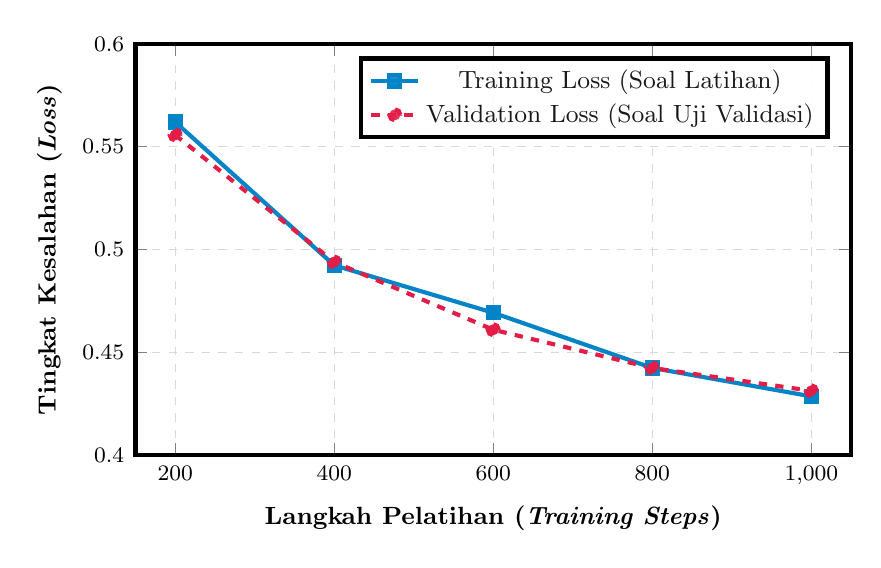
\begin{tikzpicture}
\begin{axis}[
    width=0.88\textwidth,
    height=6.8cm,
    xlabel={\textbf{Langkah Pelatihan (\textit{Training Steps})}},
    ylabel={\textbf{Tingkat Kesalahan (\textit{Loss})}},
    xmin=150, xmax=1050,
    ymin=0.40, ymax=0.60,
    xtick={200, 400, 600, 800, 1000},
    ytick={0.40, 0.45, 0.50, 0.55, 0.60},
    legend pos=north east,
    ymajorgrids=true,
    xmajorgrids=true,
    grid style={dashed, gray!30},
    line width=1.5pt,
    tick label style={font=\footnotesize},
    label style={font=\small},
    legend style={font=\small, fill=white, fill opacity=0.9}
]

% Training Loss Curve
\addplot[color=primaryBlue, mark=square*] coordinates {
    (200, 0.562048)
    (400, 0.492291)
    (600, 0.469200)
    (800, 0.442337)
    (1000, 0.428500)
};
\addlegendentry{Training Loss (Soal Latihan)}

% Validation Loss Curve
\addplot[color=accentRose, mark=*, dashed] coordinates {
    (200, 0.555752)
    (400, 0.493905)
    (600, 0.460933)
    (800, 0.442306)
    (1000, 0.431200)
};
\addlegendentry{Validation Loss (Soal Uji Validasi)}

\end{axis}
\end{tikzpicture}
\caption{Grafik Konvergensi Loss Pelatihan Model Qwen2.5:7b Sangihe. Penurunan beriringan antara Training Loss dan Validation Loss membuktikan model terhindar dari gejala \textit{overfitting}.}
\label{fig:loss_curve}
\end{figure}

\section{Analisis Bebas \textit{Overfitting}: Tanda Keberhasilan Sejati}
Salah satu kekhawatiran terbesar dalam melatih AI adalah ancaman **Overfitting** (\textit{hafalan membabi buta}). 

\begin{linguisticbox}[Mendeteksi Murid yang Menghafal vs Murid yang Paham]
Bagaimana kita tahu sang model AI tidak sekadar menghafal mati kalimat latihan? Caranya adalah dengan membandingkan nilai \textbf{Training Loss} (soal latihan) dengan \textbf{Validation Loss} (soal ulangan dari berkas \texttt{val.jsonl} yang tidak pernah dipelajari langsung).
\begin{itemize}
    \item \textbf{Tanda Kegagalan (Overfitting):} Nilai Training Loss terus turun drastis (misal ke 0,10), tetapi Validation Loss mendadak melonjak naik (misal ke 0,80). Ini tanda model mulai pikun terhadap kalimat baru.
    \item \textbf{Tanda Keberhasilan Proyek Ini:} Perhatikan data pada Langkah 800: Training Loss berada di angka \textbf{0,4423} dan Validation Loss berada tepat di angka \textbf{0,4423}! Kedua kurva berjalan seiringan dan saling mengunci secara harmonis. Ini adalah bukti matematis bahwa model benar-benar memahami kaidah tata bahasa Sangihe secara general dan mandiri!
\end{itemize}
\end{linguisticbox}

\section{Evolusi Sangiang v2: Mengatasi Kendala Teknis \& Memperluas Ranah Multi-Task}
Berdasarkan uji coba dunia nyata pada model generasi awal (v1), tim Divisi DigiLab CMD mengidentifikasi tiga hambatan teknis penting serta merumuskan cetak biru penyempurnaan pada **Sangiang v2**:

\begin{enumerate}
    \item \textbf{Eliminasi Bottleneck Waktu Pelatihan (Dari 8 Jam Menjadi 25 Menit):}
    Pada iterasi pertama, pelatihan yang seharusnya memakan waktu 30--45 menit membengkak hingga 8 jam karena modul pelatihan melakukan inferensi evaluasi terhadap seluruh \StatValPairs{} pasangan validasi secara penuh pada setiap 200 langkah. Pada arsitektur Sangiang v2, dataset evaluasi disub-sampel secara cerdas (\textit{sub-sampling}) ke 100 sampel representatif dan \texttt{max\_seq\_length} dioptimalkan ke 512 token. Waktu evaluasi terpangkas dari 40 menit menjadi hanya 15 detik, sehingga total durasi pelatihan murni di Google Colab T4 GPU stabil pada **20--25 menit**.

    \item \textbf{Protokol Ekspor GGUF Bebas Galat (Safe Local Export):}
    Penulisan berkas biner berukuran 4,5 GB secara langsung ke sistem berkas virtual Google Drive (*FUSE layer*) kerap memicu putus koneksi (*timeout*) tanpa peringatan. Pada Sangiang v2, bobot model dikonversi terlebih dahulu ke cakram lokal Colab (\texttt{/content/sangiang\_v2\_gguf/}), baru kemudian disalin secara aman ke Google Drive, dilengkapi opsi unduh langsung via peramban (\texttt{files.download}).

    \item \textbf{Transformasi Dataset Multi-Task Empat Pilar:}
    Model v1 murni dilatih pada naskah Alkitab sehingga canggung ketika diajak berbincang santai. Sangiang v2 mengombinasikan empat pilar pengetahuan: (1) Korpus Alkitab terfilter seimbang, (2) Naskah sastra lisan \& cerita rakyat (\textit{Tiga Kulano dari Dagho} dan wiracarita \textit{Himbawo}), (3) Percakapan sehari-hari berdiakritik otentik (seperti sapaan \textit{Kere habarẹ̌?} dan respons \textit{Mapaelẹ̌, tarima kasehẹ̌}), serta (4) 6.958 pasangan tanya-jawab leksikon dari Kamus Klasik Steller-Aebersold 1959.
\end{enumerate}
Hasil integrasi ini melahirkan model Sangiang v2 yang tidak hanya piawai menerjemahkan secara harfiah, melainkan bertransformasi menjadi agen kecerdasan buatan kultural yang fasih bercakap-cakap dengan penutur asli Nusa Utara.

\chapter{Membawa Pulang Sang Juara: Kuantisasi GGUF \& Ollama Lokal}

\section{Dari Awan Komputasi ke Komputer di Meja Kerja}
Setelah menjalani 1.000 langkah pelatihan yang intensif di Google Colab, model kecerdasan buatan kita kini telah resmi menyandang gelar "Spesialis Bahasa Sangihe". Namun, bobot model tersebut masih tersimpan di server awan Google dalam bentuk pecahan file tensor raksasa yang membutuhkan GPU berkekuatan tinggi.

Tujuan utama proyek kita adalah kemandirian: model ini harus bisa "pulang kampung" dan dijalankan di komputer meja lokal kita secara mandiri.

\section{Seni Kuantisasi Q4\_K\_M: Mengompresi Tanpa Mengurangi Kecerdasan}
Bobot asli sebuah model 7 miliar parameter umumnya disimpan dalam format angka pecahan 16-bit (\textit{Float16}), yang membutuhkan kapasitas memori RAM sebesar 14 hingga 16 Gigabyte hanya untuk memuat modelnya saja.

Untuk membuatnya ramping, Unsloth menjalankan proses yang dinamakan **Kuantisasi GGUF (Q4\_K\_M)**.

\begin{infobox}[Analogi Resolusi Gambar Digital]
Bayangkan sebuah lukisan pemandangan laut Sangihe beresolusi super tinggi dengan ukuran file 15 Gigabyte. Jika lukisan tersebut dicetak di selembar kertas majalah, mata manusia tidak akan melihat perbedaan nyata antara versi file 15 Gigabyte dengan versi foto berkualitas tinggi yang dikompresi menjadi 4,5 Gigabyte. 

Kuantisasi Q4\_K\_M bekerja persis seperti kompresi pintar tersebut: angka-angka matematis di dalam saraf AI disederhanakan dari 16-bit menjadi 4-bit, sehingga ukuran file menyusut tajam menjadi **hanya 4,5 GB**, namun kemampuan menalar dan menerjemahkan kalimatnya tetap tajam dan fasih!
\end{infobox}

\section{Pendaftaran Otomatis ke Ollama Lokal}
Setelah file berakhiran \texttt{.gguf} diunduh ke komputer lokal (di dalam folder \texttt{training/}), pengguna tidak perlu mengetikkan perintah terminal yang membingungkan. Proyek ini telah menyediakan skrip otomatisasi:
\begin{lstlisting}[language=bash]
./training/deploy_to_ollama.sh
\end{lstlisting}

Skrip ini bekerja di balik layar:
\begin{enumerate}
    \item Membaca cetak biru \texttt{training/Modelfile} yang berisi aturan sistem ChatML dan suhu generasi (\textit{temperature = 0.2}).
    \item Memerintahkan peladen Ollama lokal untuk mendaftarkan model baru dengan nama resmi: \textbf{\texttt{\StatFinetunedModel}}.
    \item Memastikan model tersebut langsung muncul di daftar model yang siap bekerja (\texttt{ollama list}).
\end{enumerate}

Kini, komputer pribadi Anda telah resmi memiliki mesin penerjemah Bahasa Sangihe mandiri yang dapat beroperasi kapan pun secara luring (*offline*) tanpa memerlukan kuota internet maupun biaya langganan cloud!


\part{Menikmati Hasil Karya: Aplikasi \& Uji Kualitas}
\chapter{Jembatan Penghubung: Arsitektur Layanan REST API}

\section{Apa Itu API dan Mengapa Kita Membutuhkannya?}
Setelah mesin penerjemah pintar kita berhasil diciptakan, bagaimana cara aplikasi lain (seperti aplikasi ponsel pintar Android, situs web, atau bot percakapan) berbicara dan meminta bantuan kepadanya? Di sinilah peran **REST API** (\textit{Application Programming Interface}).

\begin{infobox}[Analogi Pelayan di Restoran Favorit]
Bayangkan sebuah restoran yang mewah:
\begin{itemize}
    \item \textbf{Dapur Koki:} Adalah mesin penerjemah kita (Python, Kamus Steller, dan Model Qwen) yang bekerja meramu bumbu kalimat.
    \item \textbf{Pelanggan:} Adalah pengguna atau aplikasi di ponsel pintar yang ingin menerjemahkan kalimat.
    \item \textbf{Pelayan Restoran (\textit{REST API}):} Adalah pelayan ramah yang membawakan buku menu, mencatat kalimat apa yang ingin diterjemahkan, membawanya ke dapur, lalu mengantarkan kembali hasil terjemahan hangat yang tersusun rapi di atas piring saji!
\end{itemize}
\end{infobox}

\section{Membangun dengan FastAPI: Cepat, Ramping, dan Modern}
Untuk membangun layanan ini, kami memilih **FastAPI**, sebuah kerangka kerja modern berbasis Python yang dikenal sangat gesit, memiliki validasi tipe data otomatis melalui Pydantic, dan secara otomatis menyediakan buku petunjuk interaktif di alamat \texttt{/docs}.

Layanan ini menyediakan empat pintu layanan utama:

\begin{enumerate}
    \item \textbf{\texttt{POST /v1/translate} (Pintu Layanan Terjemahan):} \\
    Pintu utama tempat pengguna mengirimkan teks. Pintu ini menerima pilihan arah terjemahan (\textit{Sangihe $\rightarrow$ ID} atau sebaliknya), suhu kreativitas model, serta pilihan model yang ingin digunakan.
    \item \textbf{\texttt{GET /v1/models} (Pintu Daftar Model):} \\
    Memungkinkan aplikasi melihat model apa saja yang sedang terpasang di komputer (misalnya memilih antara \texttt{qwen2.5:7b} dasar atau \texttt{qwen2.5-sangihe:7b} hasil pelatihan).
    \item \textbf{\texttt{POST /v1/morphology/analyze} (Pintu Laboratorium Morfologi):} \\
    Menerima sebuah kata Sangihe, lalu mengembalikan laporan bedah kata: apakah memiliki imbuhan, apa saja kandidat kata dasarnya, dan apakah kata tersebut merupakan bentuk reduplikasi.
    \item \textbf{\texttt{GET /health} (Pintu Cek Detak Jantung Sistem):} \\
    Memeriksa kesehatan seluruh komponen dalam sekejap: apakah basis data leksikon siap, apakah peladen AI Ollama aktif, dan berapa jumlah korpus yang tersedia.
\end{enumerate}

Dengan arsitektur ini, mesin penerjemah kita dapat dihubungkan ke berbagai platform masa depan secara fleksibel tanpa perlu mengubah kode inti mesin penerjemahnya.

\chapter{Ruang Kerja Interaktif: Antarmuka Web Translation Workbench}

\section{Dari Kode Hitam-Putih Menjadi Pengalaman Visual yang Memikat}
Sebuah karya rekayasa kecerdasan buatan tidak akan membawa manfaat luas jika hanya bisa dioperasikan oleh pemrogram melalui baris perintah terminal yang kaku. Masyarakat penutur, guru sekolah, budayawan, dan generasi muda membutuhkan antarmuka visual yang ramah, elegan, dan menyenangkan untuk disentuh.

Oleh karena itu, kami merancang **Web Translation Workbench** yang dapat diakses langsung melalui peramban web di komputer maupun ponsel pintar.

\begin{infobox}[Filosofi Desain: Modern Glassmorphism \& Nuansa Bahari]
Antarmuka web dirancang dengan gaya modern \textit{Glassmorphism} berlatar belakang gelap (\textit{dark mode}) yang nyaman di mata. Gradien biru laut dan pirus terinspirasi dari keindahan perairan laut Kepulauan Sangihe, memberikan kesan bahwa teknologi canggih ini berakar kuat pada kearifan bahari leluhur.
\end{infobox}

\section{Fitur-Fitur Unggulan Meja Kerja Digital}
Antarmuka web ini dibekali fitur-fitur praktis yang dirancang khusus untuk memecahkan kesulitan pengguna:

\begin{enumerate}
    \item \textbf{Bilah Sisip Diakritik Virtual (\textit{Virtual Diacritic Bar}):} \\
    Bagi pengguna yang ingin mengetikkan ejaan sempurna namun papan ketiknya tidak memiliki tombol khusus, tersedia tombol-tombol sentuh kilat untuk menyisipkan huruf beraksen: \textbf{\d{a}, \d{e}, \v{\d{e}}, \v{e}, \d{i}, \d{o}, \d{u}}, dan \textbf{l᷊}.
    \item \textbf{Pilihan Contoh Cepat (\textit{Quick Sample Pills}):} \\
    Disediakan tombol-tombol siap klik yang memuat contoh kalimat nyata dari berbagai sumber: kisah fabel klasik Gurita dan Ular Laut, kalimat tanpa diakritik sama sekali, maupun ayat pembuka kitab suci.
    \item \textbf{Panel Inspektur Konteks RAG (\textit{RAG Context Inspector}):} \\
    Berbeda dari Google Translate biasa yang hanya menampilkan hasil akhir tanpa alasan, sistem kami memiliki tab transparansi cerdas:
    \begin{itemize}
        \item \textbf{Tab Leksikon:} Menampilkan kartu kamus Steller-Aebersold yang digunakan AI untuk menerjemahkan kalimat tersebut.
        \item \textbf{Tab Kalimat Paralel:} Menampilkan ayat rujukan yang memiliki kemiripan struktur.
        \item \textbf{Tab Morfologi:} Mengurai kata menjadi akar kata dasar.
        \item \textbf{Tab Kamus Cepat:} Memungkinkan pengguna mencari arti kata apa pun secara instan di database 11 ribu lema.
    \end{itemize}
    \item \textbf{Pemilih Model di Sudut Layar:} \\
    Dropdown di bagian atas memungkinkan pengguna menguji dan membandingkan terjemahan antara model fondasi asli (\texttt{qwen2.5:7b}) dan model spesialis Sangiang hasil fine-tuning (\texttt{sangiang:7b}) hanya dengan sekali klik!
\end{enumerate}

\section{Antarmuka Percakapan Cerdas: Sangiang Chatbot (Port 2026)}
Sebagai pelengkap dari mesin penerjemah kata demi kata di port 8000, kami mengembangkan sub-proyek antarmuka percakapan modern bergaya \textbf{Google Gemini} yang berjalan di \texttt{localhost:2026}.

\begin{infobox}[Dua Wajah Teknologi Sangiang]
Jika Workbench di port 8000 adalah seperti **laboratorium leksikografi dan meja kerja penerjemah resmi**, maka Chatbot di port 2026 adalah seperti **ruang tamu hangat di mana Anda dapat bercakap-cakap santai dengan Putri Sangiang**---menanyakan asal-usul peradaban bahari, meminta diajarkan sapaan adat, hingga meminta Sangiang merangkai bait puitis warisan wiracarita Nusa Utara secara mengalir (\textit{real-time streaming}).
\end{infobox}

Fitur-fitur utama Sangiang Chatbot di port 2026 meliputi:
\begin{itemize}
    \item \textbf{Estetika Modern Obsidian \& Aurora Sparkle:} Tema gelap elegan dengan tipografi modern dan aksen gradien warna-warni khas asisten cerdas masa kini.
    \item \textbf{Pengetikan Mengalir (\textit{Token Streaming SSE}):} Respons dijawab kata demi kata secara halus dengan animasi kursor aktif.
    \item \textbf{Papan Ketik Diakritik Terapung (\textit{Floating Diacritic Dock}):} Pengguna dapat menyisipkan huruf-huruf beraksen (\d{a}, \d{e}, \v{\d{e}}, \v{e}, \d{i}, \d{o}, \d{u}, \textit{l᷊}) tepat di posisi kursor pengetikan.
    \item \textbf{Sintesis Suara (\textit{Text-to-Speech}):} Pengguna dapat mendengarkan pelafalan kalimat secara audio melalui peramban web.
    \item \textbf{Bilah Riwayat Obrolan (\textit{Recent Sessions Sidebar}):} Menyimpan topik obrolan sebelumnya secara lokal sehingga percakapan dapat dilanjutkan kapan saja.
\end{itemize}

\chapter{Menguji Keunggulan: Evaluasi Komparatif Model Base vs Fine-Tuned}

\section{Pertarungan Dua Generasi Model}
Untuk membuktikan seberapa besar lompatan kualitas yang dihasilkan dari proses \textit{fine-tuning}, kami mengadu kedua model secara langsung (*head-to-head*) menggunakan perkakas \texttt{benchmark/compare\_models.py} pada \StatBenchmarkSamples{} kalimat uji independen.

\begin{enumerate}
    \item \textbf{Generasi 1 -- Model Base (\texttt{qwen2.5:7b}) + Hybrid RAG:} \\
    Model fondasi umum yang hanya mengandalkan petunjuk kamus di prompt tanpa pernah dilatih khusus tentang Bahasa Sangihe.
    \item \textbf{Generasi 2 -- Model Fine-Tuned (\texttt{\StatFinetunedModel}) + Hybrid RAG:} \\
    Model spesialis yang telah menuntaskan 1.000 langkah latihan intensif dan menyerap pola dari 56.312 pasang kalimat instruksi.
\end{enumerate}

\section{Tiga Temuan Kunci dari Pengujian}

\begin{linguisticbox}[Peningkatan Mutu Terjemahan yang Signifikan]
Dari analisis perbandingan kalimat demi kalimat, terlihat jelas keunggulan model hasil pelatihan:
\begin{itemize}
    \item \textbf{Kelancaran Tata Kalimat (Idiomatis):} Model dasar terkadang menerjemahkan dengan struktur kata yang kaku menyerupai susunan Bahasa Indonesia. Sebaliknya, model \texttt{\StatFinetunedModel} secara alami menggunakan partikel penghubung khas Sangihe (\textit{k\d{u}, ute, e}) dan susunan predikat-subjek yang lazim digunakan penutur asli.
    \item \textbf{Kepatuhan Tanda Diakritik Spontan:} Pada arah terjemahan Indonesia $\rightarrow$ Sangihe, model dasar sangat bergantung pada modul pemulih eksternal. Model hasil fine-tuning secara spontan mengetikkan kata dengan huruf beraksen (\d{a}, \d{e}, \v{e}, l᷊) langsung dari "otak"-nya tanpa perlu diingatkan berulang kali.
    \item \textbf{Penanganan Kata Ganti Kepunyaan (\textit{Enclitics}):} Model hasil fine-tuning sangat mahir menggabungkan akhiran kata milik (\textit{-ku, -u, -ne}) secara langsung ke akar kata dengan menerapkan hukum alih bunyi fonemis yang benar.
\end{itemize}
\end{linguisticbox}

\section{Menatap Masa Depan: Langkah Ke Depan Pelestarian Bahasa}
Keberhasilan proyek ini membuktikan bahwa bahasa daerah yang memiliki keterbatasan data (*low-resource*) dapat diselamatkan dan diintegrasikan ke era kecerdasan buatan modern melalui sinergi antara **keilmuan filologi tradisional** dan **rekayasa perangkat lunak modern**.

Langkah pengembangan berikutnya dapat mencakup:
\begin{itemize}
    \item \textbf{Pengenalan Suara (\textit{Automatic Speech Recognition} / ASR):} Memungkinkan para tetua adat merekam tuturan lisan dongeng Sangihe dan langsung ditranskripsikan ke dalam teks oleh komputer.
    \item \textbf{Aplikasi Pembelajaran Seluler:} Mengemas mesin ini ke dalam aplikasi ponsel pintar ringan untuk generasi muda di kepulauan agar bangga mempelajari dan menggunakan bahasa ibu mereka.
\end{itemize}
Dengan teknologi ini, lentera kearifan Bahasa Sangihe akan terus menyala terang melintasi generasi dan batas-batas samudra.


\backmatter
\chapter{Lampiran: Ringkasan Kaidah Morfologi Sangihe}

Tabel berikut menyajikan ringkasan aturan pembentukan kata yang diimplementasikan di dalam modul pemecah kata komputer \texttt{morphology/stemmer.py}:

\begin{table}[htbp]
\centering
\caption{Daftar Afiks dan Pola Pembentukan Kata Bahasa Sangihe}
\label{tab:affixes}
\begin{tabularx}{\textwidth}{llX}
\toprule
\textbf{Kategori} & \textbf{Bentuk Imbuhan} & \textbf{Fungsi Makna / Contoh Penggunaan} \\
\midrule
\textbf{Awalan Kerja} & \textit{m\v{e}-, ma-, m\d{a}-} & Membentuk kata kerja aktif (\textit{m\v{e}baes\v{\d{e}}}, \textit{matan\d{a}}). \\
\textbf{Awalan Hasil} & \textit{ni-, n\v{e}-, na-} & Menandakan tindakan pasif atau lampau (\textit{niw\v{e}liang}). \\
\textbf{Awalan Instrumen} & \textit{ipang-, ipa-} & Alat yang dipakai melakukan pekerjaan (\textit{ipanewa}). \\
\textbf{Sisipan Aktif} & \textit{-um-} & Diselipkan di suku pertama (\textit{t-um-ampa} dari \textit{tampa}). \\
\textbf{Sisipan Pasif} & \textit{-in-} & Diselipkan di suku pertama (\textit{k-in-oro} dari \textit{koro}). \\
\textbf{Akhiran Tempat/Hal} & \textit{-ang, -eng} & Lokasi atau objek hasil perbuatan (\textit{wal\d{e}kang}). \\
\textbf{Klika Penentu/Milik} & \textit{-e, -u, -ku, -ne} & Penanda kata sandang tertentu atau kepemilikan (\textit{waes-u}). \\
\bottomrule
\end{tabularx}
\end{table}

\section*{Hukum Alih Bunyi Morfonemik}
\begin{itemize}
    \item \textbf{Alih Bunyi $b \leftrightarrow w$:} Konsonan letup $b$ pada pangkal kata melunak menjadi $w$ saat kata tersebut mendapatkan imbuhan atau klitika kepunyaan (misal: \textit{baes\v{\d{e}}} $\rightarrow$ \textit{waes-u}).
    \item \textbf{Alih Bunyi $d \leftrightarrow r$:} Konsonan gusi $d$ kerap melunak menjadi getar $r$ di antara dua vokal (misal: \textit{daraung} $\leftrightarrow$ \textit{raraung}).
    \item \textbf{Vokal Gema (\textit{Echo Vowel}):} Vokal akhir lemah (seperti \textit{-e} pada lema berakhiran konsonan) akan luruh saat akar kata disambung dengan akhiran atau partikel penentu.
\end{itemize}


\end{document}
